%% ----------------------------------------------------------------
%% Introduction.tex
%% ---------------------------------------------------------------- 
% PR-Akshay
\chapter{System Design} \label{Chapter:System Design}
% Need an introduction to the system design - referencing to system diagrams generated
Following the brief outlined in \ref{0_2_project_brief}, the system diagram shown in Figure \ref{fig_system_diagram_full} allows the system to be split into three different stages, with a fourth stage for any application derived from the data and from any classifications made by the ML Model developed. 
\begin{enumerate}
    \item Data Collection and Transformation
    \item Localised Processing, Storage and Classification
    \item Cloud Based Processing, Storage and Inference
    \item Over-the-top Application using ML Model Outputs and Input Data
\end{enumerate}



\begin{figure}[ht]
    \label{fig_system_diagram_full}
    \centering
    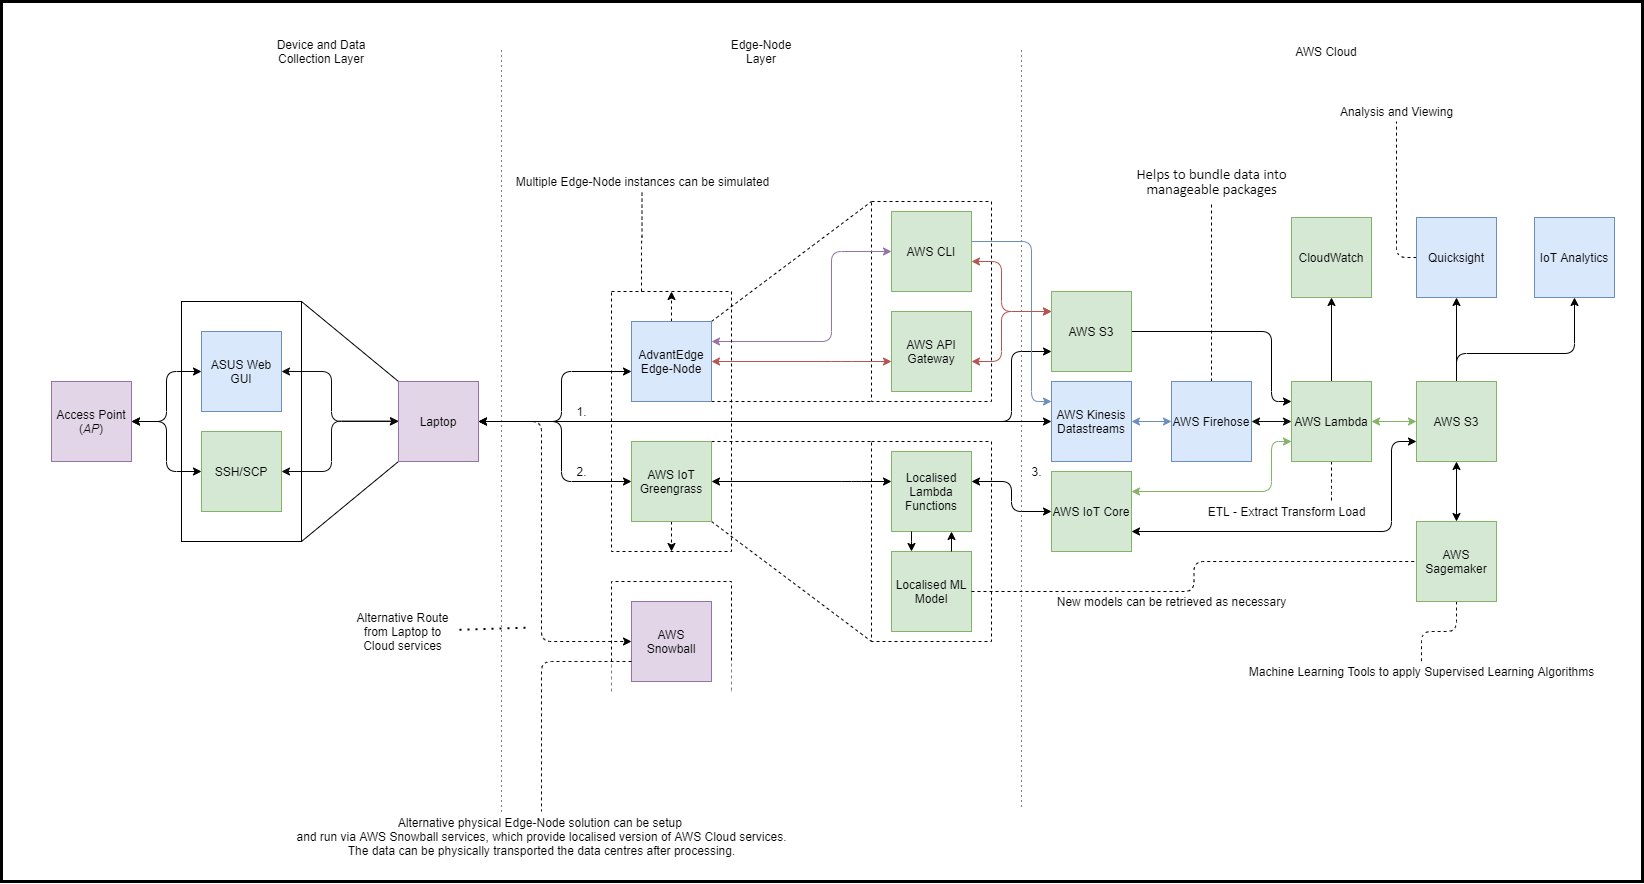
\includegraphics[width=1\linewidth]{pages/Chapter3/Chapter 3 images/block_system_diagram_v2.png}
    \caption{Full System Diagram - The full scale diagram can be seen in Appendix \ref{appendix:full_scale_system_diagram}}
\end{figure}

From these 4 stages, the system design can be understood. All data is collected from the access point, which for this project is ASUS Rog AX11000 Router, which is connected to a laptop and is responsible for data retrieval. The laptop in this wireless pipeline is an end-user connected to some access-point. The project then explores data transportation through several data pipe-lining methods..
\begin{itemize}
    \item Data is sent directly to the cloud from the Laptop after data is compressed into a smaller and better format for transport.
    \item Data is sent to a local Edge Node containing processing and ML models to process data and all analytics and results are computed direclty on the Edge Node.
    \item Data is sent to the cloud from the laptop via the Edge Node. Comparisons in latency of response can easily be drawn from this.
\end{itemize}

In the following few sections, the report will explore each of these stages metnionted above as well as how data will be processed in each pipeline path.

% PR - Eu Jin   -COMPLETE 1
\section{Data Collection and Transformation}
\label{data_collection_design}
% Need to discuss db -> json files
% Compression of json files into 1 json file
% Conversion into format for ML format
% \usepackage{arydshln}

Following on from the research conducted into the wireless network parameters that can be recorded using the ASUS ROG router (Section \ref{section:WirelessTelemetryResearch}), the next step is to design the system to utilise all relevant data. 

\subsection{Data Categorisation}
\label{Section: Data Categorisation}

\begin{figure} [ht]
    \centering
    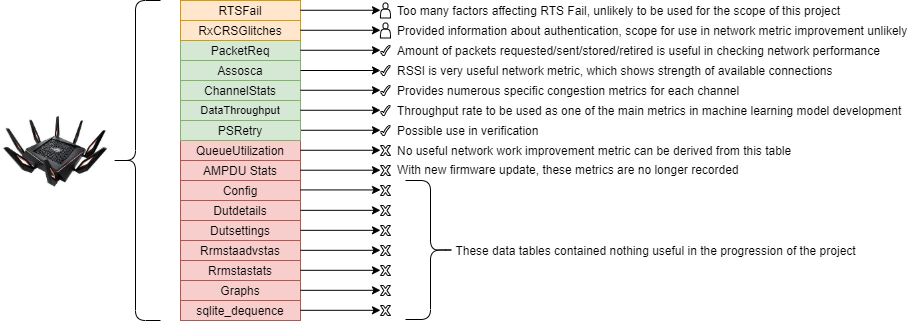
\includegraphics[width=1\linewidth]{pages/Chapter3/Chapter 3 images/router_data-Datasets-Usefulness.png}
    \caption{Database file table categorisation. Full  scale  diagram  can be seen in Appendix A Section \ref{appendix:ASUS router datatable}.}
    \label{fig_ASUSDatatables}
\end{figure}

The first stage of this process is to categorise the data into three sections; relevant data to be used in machine learning development \& deployment, data with potential but specific use cases and redundant data. The database (.db) file generated by the ASUS router, catalogs the data parameters into separate data tables as shown on the left hand side of Figure \ref{fig_ASUSDatatables}. The tables marked in red are either redundant data providing no useful insights into network performance or data through  which no meaningful information can be derived. Tables marked orange present beneficial information with potential for use but are not within the scope of this project. hence will not be further considered. Tables marked green all provide useful information through which network characteristics can be analysed and will be further studied for the purposes of Machine Learning model and OTT application development.  


The next step in this system design process was to understand how each table in the .db database file was organised. Each table starts with a column titled "rowID" labeled 1 - 3, which correspond to the current operational frequency band (5GHz-1, 2.4GHz and 5GHz-2 respectively). Then the individual data parameters are classified under a column titled "GraphrowID" labeled 1 - 17 which define what each dataset in the table represents. Table \ref{table:GUIData} shows the GraphrowID values and their corresponding parameter, unit and table name. 


\begin{table}[h]
\centering

\begin{tabular}{:l:l:l:l:} 
\hline
\multicolumn{1}{|l|}{\textbf{GraphrowID}} & \multicolumn{1}{l|}{\textbf{Parameters}} & \multicolumn{1}{l|}{\textbf{Units}} & \multicolumn{1}{l|}{\textbf{Table Name}}  \\ 
\hline
1                                         & Congestion                               & Percentage                          & ChannelStats                              \\
2                                         & Chanim Statistics                        & Count                               & ChannelStats                              \\
3                                         & Rx CRS Glitches                          & Count                               & RxCRSGlitches                             \\
4                                         & Bad PLCP~                                & Count                               & RxCRSGlitches                             \\
5                                         & Bad FCS                                  & Count                               & RxCRSGlitches                             \\
6                                         & Packet Requested                         & Count                               & PacketRequested                           \\
7                                         & Packet Stored~                           & Count                               & PacketRequested                           \\
8                                         & Packet Dropped                           & Count                               & PacketRequested                           \\
9                                         & Packet Retired                           & Count                               & PacketRequested                           \\
10                                        & Queue Utilisation~                       & Count                               & QueueUtilisation                          \\
11                                        & Queue Length Per Precedence              & Count                               & QueueUtilisation                          \\
12                                        & Data Throughput~                         & Mbits/s                             & DataThroughput                            \\
13                                        & Physical Rate~                           & Mbits/s                             & DataThroughput                            \\
14                                        & RTS Fail~                                & Count                               & RTSFail                                   \\
15                                        & Retry Drop~                              & Count                               & RTSFail                                   \\
16                                        & PS Retry                                 & Count                               & PSRetry                                   \\
17                                        & Acked                                    & Count                               & PSRetry                                   \\
%\hdashline
\end{tabular}
\caption{ASUS ROG Router Data Table\\}
\label{table:GUIData}
\end{table}

\subsection{Database File Conversion}
\label{Section: Database File Conversion}

Now with a better understanding of all the parameters that can be recorded through the ASUS router and having established which parameters will be further considered, the next step is to convert the database file into a more appropriate format. A .db file is typically used on mobile devices and is not intended to be opened or edited manually \cite{dbFiles}, because of this the .db file format is not suitable in the development of the telemetry pipeline plus it is not compatible with AWS. For this three other file formats were considered CSV, XML and JSON. The CSV (Comma Separated Value) format is a delimited text file which uses commas to separate out values. Each line of the file is a record and each record is compromised of one or more fields separated by commas. CSV files are best used to represent data in which each record has an identical list of fields with a single relation, and databases which have multiple relations cannot be exported to a single file. Hence the best use case is when the data has a strict tabular structure and when very large databases are required to be transferred between programs. XML (Extensible Markup Language) is a self-defining file format, meaning the structure of the data is embedded within the data itself, therefore when the data arrives at the destination there is no need to pre-build the structure. Due to its platform independent nature XML simplifies the data transfer process as there is no further conversion necessary when transferring between different systems. However, the syntax for XML is verbose and the redundancy in the syntax results in higher storage and transportation costs. JSON (JavaScript Object Notation) is a lightweight text based file and data interchange format which uses human-readable text to store data objects. It is primarily used to transmit data between a server and web application due to the fact that JSON provides easy parsing and faster execution of the data. 

With the three file formats researched and better understood, the decision was made to convert the .db file into the JSON format for further use in the development of the telemetry pipeline. CSV was not chosen as it does not provide the ability to have relational databases. Also XML was not chosen as it added redundancy to the data with its verbose syntax, hence it would not be appropriate in a system where efficiency and low latency was critical to its operation. Furthermore, with the ability of JSON to use less data resulting in increased parsing and execution speeds it was chosen as the main file format in this project. 


\subsection{JSON File Compression}
\label{Section: JSON File Compression}


With the way in which the .db file generated by the ASUS router is organised, each relevant data table needs to be read into separately. This means that in the conversion stage, every data table that is converted will produce its own JSON file. These individual JSON files are to be used in the direct upload to the S3 data storage, where it will be further processed on the cloud. However, on the edge node side of the system these distinct JSON files must be combined and compressed into a single file for further use. As well as this further compression and removal of unnecessary data is required for use in Machine Learning model. 

\subsubsection{JSON Conversion Keys for Each Table}

\textbf{\underline{ChannelStats}}

[rowID, TimeStamp, Channel, tx, inbss, obss, nocat, nopkt, doze, txop, goodtx, badtx, glitch, plcp, noise, idle]

\textbf{\underline{Assocsta}}

[rowID, TimeStamp, "MAC", RSSI, PhyRate]

\textbf{\underline{DataThroughput}}

[rowID, GraphrowID, "MAC", TimeStamp, "XAxis", " Data Throughput/Physical Rate"]

\textbf{\underline{PacketRequested}}

[rowID, GraphrowID, "MAC", TimeStamp, "XAxis", " Packet Requested/Stored/Dropped/Retired"]

\textbf{\underline{PSRetry}}

[rowID, GraphrowID, "MAC", TimeStamp, "XAxis", " PS Retry/Acked"]

\subsubsection{JSON Key for Compressed File}
 
\{\\
"DeviceID - GraphrowID": "value",\\
...\\
...\\
...\\
"Channel Number - Channel Stats": "value",\\
...\\
...\\
...\\
"TimeStamp": "value"\\
\}

\subsubsection{JSON File Key for ML Model Compatibility}

['Packet Requested', 'Packet Stored ', 'Packet Retired', 'BADTX', 'GOODTX', 'TX', 'TXOP']



%  PR - Akshay - COMPLETE 1
\section{Localised Processing, Storage and Classification}
% Discuss Lambda functions deployed to the Edge and how they interact
% Discuss how web server can see data throughout the greengrass
% Discuss how AdvantEdge can help validate results within the model
% 

\subsection{Edge Node Design}
For the Edge Node design, following the research into Edge Computing in Section \ref{edge_node_technologies} and seeing that AWS IoT Greengrass is a great solution to bringing Cloud Features to the edge, it was understood that we needed processing, network capabilities, and ability to work while not interrupting the user experience. 

IoT Greengrass lets us do exactly that, IoT Greengrass is meant to be run on devices that support embedded Linux Systems, such as a Rasperry Pi, NVIDIA's Nano Jetson or Intels Atom Board to name a few. To show that our system works for any embedded system, the project places Greengrass onto a virtualised linux system running on x86\_64 architecture. However, support exists for many  other hardware architectures and OS's.
\begin{figure}[ht]
    \centering
    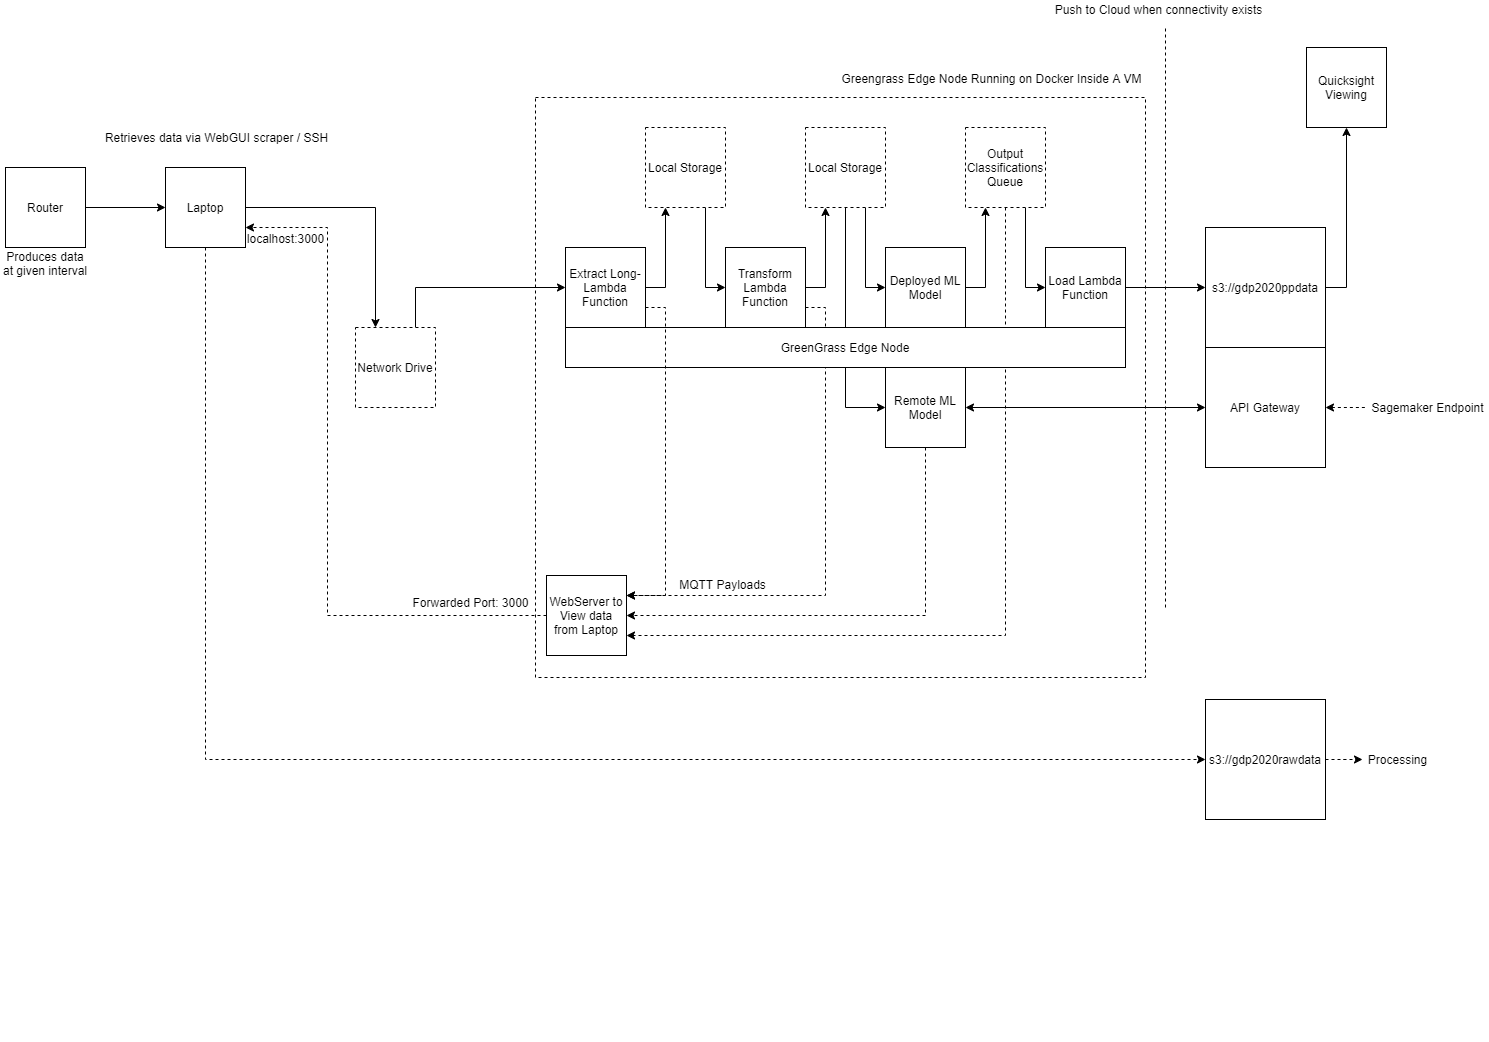
\includegraphics[width=1\linewidth]{pages/Chapter3/Chapter 3 images/greengrass_data_flow.png}
    \caption{The data flow within the Local Environment for Edge Computing -\textit{ The full scale diagram can be seen in Appendix C} [\ref{appendix:greengrass_design}]}
    \label{fig:greengrass_edge_design}
\end{figure}

From the design in Figure \ref{fig:greengrass_edge_design}, we can see how the system will function for 2 out of the 3 pipelines discussed earlier.
\begin{enumerate}
    \item Data is collected from the Router and stored in some (local) network data storage facility.
    \item This data is then retrieved by the Extract Lambda function running at the Edge and is stored locally.
    \item The Transform Lambda function will then begin the pre-processing of the data for usage and analysis.
    \item The Load Lambda function takes the pre-processed data and transfers it to the S3 Pre-Processed-Data bucket on the cloud.
    \item Pre-processed data is also taken to the ML-Inference Lambda function which uses an obtained ML Model from the Cloud for local classification of the data.
    \item Pre-processed data is used and a request is sent to the cloud for classification. Timings between Local ML-Classification and Remote ML-Classification can be compared
    \item All data is sent to a local web-server showing all timings and classifications being made by the functions described
\end{enumerate}

The first point is discussed earlier in Section \ref{data_collection_design} and how data can be collected. Point two discusses the extract function. The laptop and the edge node share a network folder within the the local environment. Data to be sent to the Edge Node will be placed into the shared folder by the laptop. In this case it is the raw data in the (.db) file format obtained from the router that is placed in the shared folder. The extract function will then take the database file and convert each data table within the database into its own JSON file.

The third item discusses the transform function. This function \textit{compresses} all the JSON files that were extracted from the database file into a single array of all data elements corresponding to a single timestamp value as described in Section \ref{data_collection_design}. 

The fourth item describes the load function. Since Edge nodes are often resource constrained in terms of hardware, either in processing power, memory available or data storage. It is often required to upload the data to the cloud upon good connectivity to ensure data is not lost and can be used for long-term analytics. The load function will then use API Gateway to securely send data to an S3 bucket to store the pre-processed data for any cloud-based processing and training of ML models. The load function allows for one of the two pipelines to be completed where data is transferred to the cloud via the Edge node rather than directly from the laptop. The sixth item is also a part of this pipeline where data can be sent to a cloud endpoint where Sagemaker has deployed a ML model to classify data. 

The fifth item discusses using a deployed ML Model that runs on the local edge node. This model is developed on the cloud using data that has been collected previously for training and verification of the model. This model can then be deployed using Greengrass where the model can be taken from any S3 bucket and then transported to the edge node. More about the model development is discussed in Section \ref{cloud_services}.

The final item in the list discusses the front-end of the Greengrass Edge node. This is a custom solution to being able to view all the data in real-time for analysis or for any OTT application to be built on top of. The data is passed around from each Lambda function using MQQT packets. Each Lambda function can subscribe to a topic. E.g. 'server/extract/data'. And on this topic, another Lambda function can publish a message for it to be read by the subscribers. These data packets can all be seen by viewers on the cloud and so other services via AWS SNS are able to subscribe to these topics and then react accordingly especially for data viewing or analytics. For this project however, a custom GUI has been designed therefore a custom OTT Application could be implemented a top of it.

\subsection{AdvantEDGE}
AdvantEDGE is a mobile edge emulation platform (MEEP) that runs on Docker and Kubernetes where all the micro-services interacted together were packaged in Docker containers before deploying in the Kubernetes pods to the AdvantEDGE for the edge scenarios testing. AdvantEDGE provides an emulation environment that enables experimentation on the edge computing technologies, applications and services. The platform facilitates exploring edge deployment models and their impact on applications and services in short and agile iterations. The user enables to define a scenario that includes:
\begin{itemize}
    \item A network topology of cloudlets, operators, wireless points of access (PoA), zones and UEs.
    \item Network characteristics for each of the elements set up including latency, jitter, packet loss and data throughput.
    \item Network and mobility events to change network characteristics and the location of UE and cloudlets during simulation run time. 
\end{itemize}

It allows the connection of real physical cloudlets and edge/fog/UE applications so that the simulation can capture the impact of the network design on its application performance. It also supports event scripting, collection of measurements in third parties such as an offline InfluxDB time series database and real time Grafana dashboards. AdvantEDGE platform and instrumented client load data into InfluxDB time series database where AdvantEDGE stores network and event measurements from deployed scenarios. Grafana dashboards were primarily used to monitor scenario execution and demonstration purposes. This combination makes it powerful platform for the edge network simulation.

\begin{figure}[ht]
    \centering
    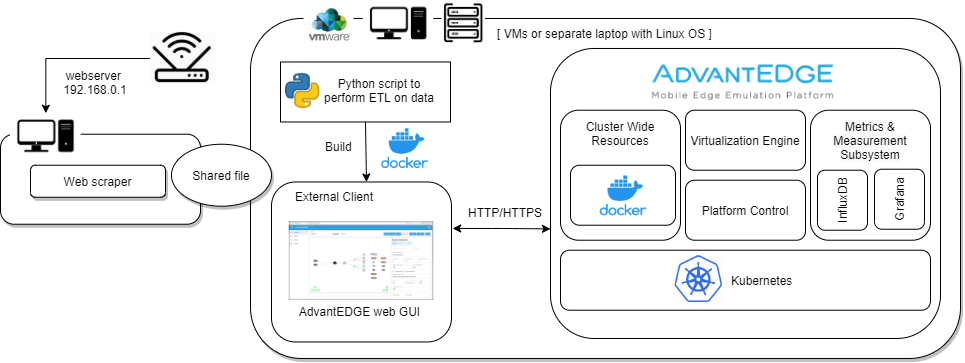
\includegraphics[width=1\linewidth]{pages/Chapter3/Chapter 3 images/System Diagram.png}
    \caption{The system diagram of edge application deployment to the AdvantEDGE}
    \label{fig:AdvantEDGE_edge_design}
\end{figure}

Figure \ref{fig:AdvantEDGE_edge_design} shows the proposed system diagram of edge application deployment on the AdvantEDGE. The data collected from the router will be accessed to the VM through shared file, where python scripts will extract these data to convert from .dB into json files, then perform transform function to compress these json files into one before loading json file into ML model for evaluation. To be able to use the functionality of the mobile edge emulation platform, these python applications will need to be built as Docker images before deploying them as a native edge application.


% PR _ Syuhada - COMPLETE 1
\section{Cloud Based Processing, Storage and Inference}
\label{cloud_services}
%Need to discuss Lambda which takes raw data to pp data bucket here
\subsection{Laptop to Cloud Pipeline}
\subsubsection{API Gateway}
In this section we discuss the entry way into the AWS Cloud. The API Gateway allows us to take any data produced the Edge location either from the end-user or the Edge nodes deployed and securely redirect them to storage and analysis endpoints. Figure \ref{fig:api_gateway_methods} shows how various URLs an be used to upload and send data to different buckets or endpoints. Usage of Sagemaker's endpoints are discussed later, but to get data from the edge to the cloud, the S3 endpoints are used by API Gateway. For example, doing a \textit{PUT} request to the provided URL from API Gateway, with the body of the request filled with the JSON object to be uploaded, would store the data file with the new Key value into the requested S3 bucket.

\begin{figure}[ht]
    \centering
    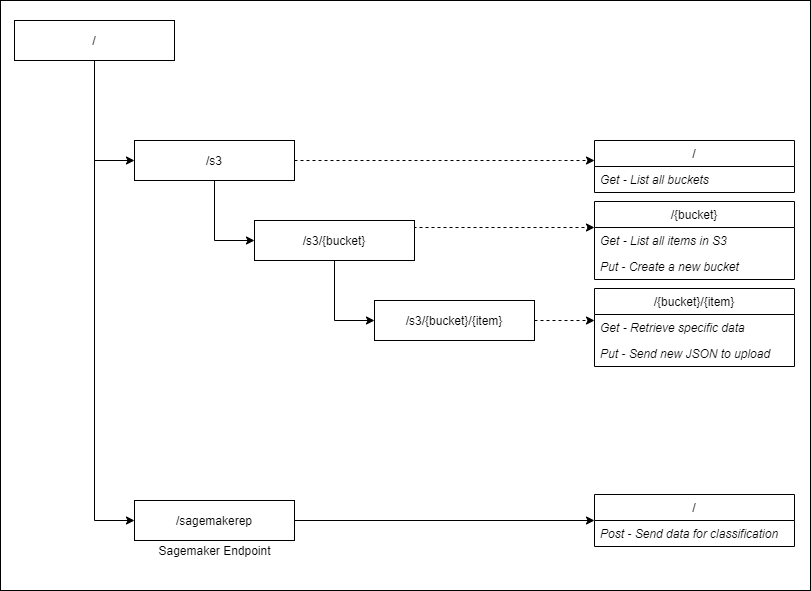
\includegraphics[width=1\linewidth]{pages/Chapter4/Chapter 4 Images/api_gateway_1.png}
    \caption{API Gateway Resources and Attached Methods}
    \label{fig:api_gateway_methods}
\end{figure}


\subsubsection{Lambda - Data Pre-processing on the Cloud}
\label{cloud_lambda}
Once the data has been prepared and the API Gateway setup, then Lambda services can be triggered to react to New Object events on S3. It can be setup such that every new object will trigger the Lambda function, however it may be the case that not all the 5 JSON files will have been uploaded as part of the Laptop to Cloud Pipeline. This would mean the pre-processing would be incomplete. One solution to this problem is for all 5 JSON files to be uploaded first and then upload a separate file with .complete file type. This was arbitrary chosen, and Lambda can be setup to trigger on only .complete files that upload to S3. This ensures that all 5 JSON files will exist before the functions searches for them. The diagram in Figure \ref{fig:s3_lambda_s3} shows this process and how it will be accomplished diagramatically.

\begin{figure}[ht]
    \centering
    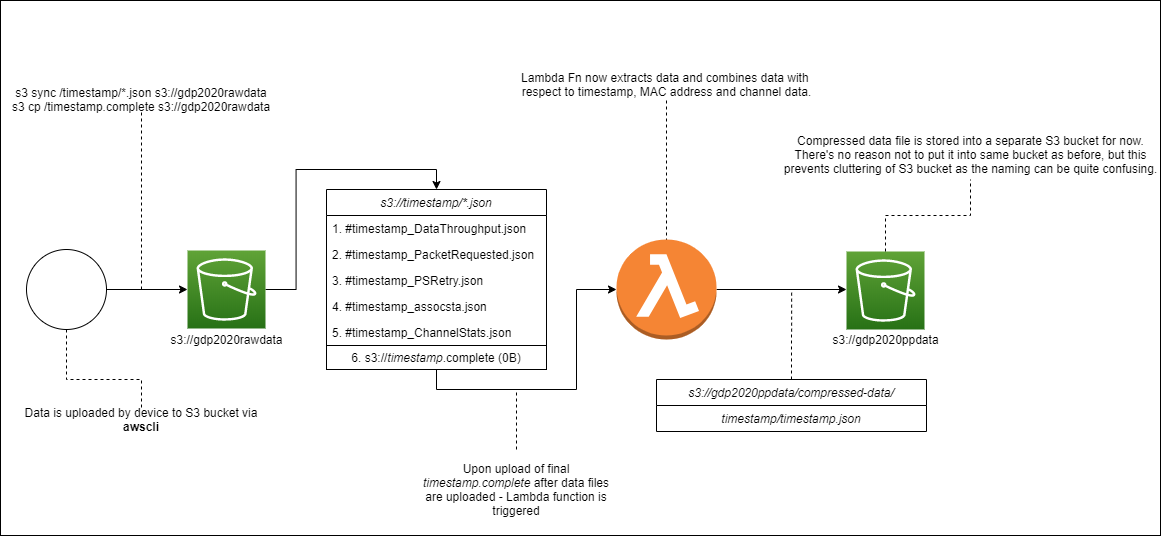
\includegraphics[width=1\linewidth]{pages/Chapter3/Chapter 3 images/S3_to_Lambda_to_S3.png}
    \caption{Triggering Lambda from S3 Uploads - \textit{The full scale diagram can be seen in Appendix E} [\ref{appendix:data_flow_from_laptop_to_cloud}]}
    \label{fig:s3_lambda_s3}
\end{figure}

\subsection{Machine Learning on the Cloud}

The following pipeline shown in \ref{appendix:ML process pipeline} summarizes the machine learning processes that will be carried out.
Firstly, the problem in building the machine learning model was identified from the telemetry data collected from the router. With careful analysis over the parameters collected, data throughput rate is chosen to create a class (target variable) labeled as data throughput strength which will be used to build the machine learning model. Data throughput rate is chosen because it is able to show the amount of data which can be received and sent within a given time span. This enables the prediction of a network performance based on the classification of data throughput strength.

\begin{figure}[ht]
    \centering
    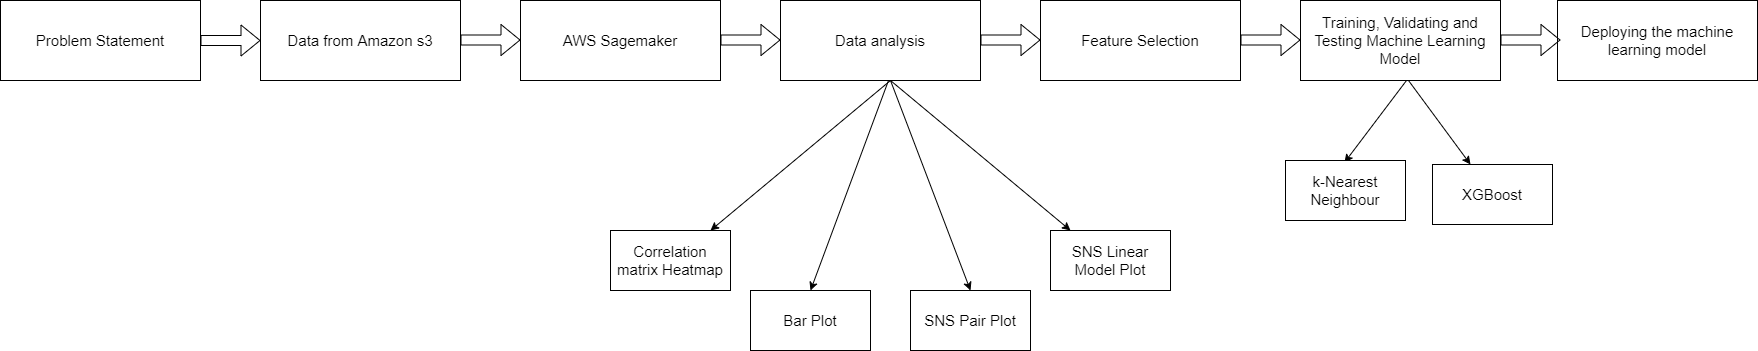
\includegraphics[width=1\linewidth]{pages/Chapter3/Chapter 3 images/Ml.PNG}
    \caption{Machine Learning Process Pipeline - \textit{Full scale diagram is in Appendix B} 
      [\ref{appendix:ML process pipeline}]}
    \label{Machine Learning Process Pipeline}
\end{figure}

The following steps to be carried out are as stated below:
\begin{itemize}
    \item Data stored as JSON files in buckets in the s3 cloud storage is imported into AWS Sagemaker with granted permission access. The code will be written in the Python programming language in JupyterLab. 
    \item Data is analysed using several methods such as correlation matrix, sns pair plots, bar plots and sns linear model plots to find correlation between parameters of the telemetry data.
    \item Useful parameters are extracted and used as features from the data analysis process. 
    \item Features selected are split into a 70:20:10 ratio for training, validating and testing the machine learning model respectively.
    \item Supervised learning algorithms such as XGBoost and k-Nearest Neighbour are used to train the ML model with hyperparameters tuned using the validating set. Testing set is used to evaluate the final performance of the machine learning model.
     \item The performance of the ML model will be evaluated with a confusion matrix with metrics such as accuracy.
    \item The ML model will be deployed after achieving a satisfying performance.
\end{itemize}

The trained machine learning model can be deployed for inference of real-time data. An endpoint will be created automatically once the model is deployed in Sagemaker. The endpoint created for the machine learning model can be invoked in the AWS cloud service.
Using Amazon API Gateway and AWS Lambda services, the endpoint can be invoked to allow the machine learning model to predict new data. To do this, a Lambda function that calls model is first created. An IAM execution role that includes a policy is chosen to give permission access to the Lambda function to invoke the model endpoint. An API gateway will then be created and deployed for the lambda function. This API will trigger an event that invokes the Lambda function where it passes data. Postman, an HTTP client for test service is used for the testing phase of the model endpoint. An invoked URL provided will be entered onto Postman with the data included in it. The prediction results on the data passed into Postman by the ML model will then be displayed on the interface. 



%  PR - Anurag - COMPLETE 1
\section{Data Analytics and the Over-the-Top Application}


%     2. ... further chapters discussing system design, build, testing, integration and further testing...






